\chapter{Fritid}


Fritiden er ikke vanskelig å fylle i en by som München. Museene og teatrene er allerede nevnt, men også konsertlokalene er mange og flotte, og det er mange verdenskjente artister som legger turen innom her når de er på turné. Alle statlige teater, operaer etc. har studentrabatt, og en kan oppleve mange flotte forestillinger for bare 5 euro. Olympiahalle og -stadion er litt større konsertarenaer for pop- og rockeartister. Det finnes også rikelig med klubblokaler som tilbyr litt mer intime konserter. Kinoer er det også nok av (også de som viser filmer på originalspråk), men det er jo de tyske kneipene som kaprer mest av fritida for mange. Det fins mange koselige kafeer og kneiper i hele byen. Vi norske bruker å være mest i bydelen Schwabing, som også karakteriseres som studentenes bydel. 


München arrangerte sommer-OL i 1972, og som et resultat av dette er tilbudene utrolig bra for studenter som liker å drive med sport og friluftsliv. I Olympiazentrum, den gamle olympiabyen, finnes det et stort sportskompleks (ZHS; Zentrale Hochschulsportanlage) som nå står til studentenes bruk. For 7,50 \euro{} pr semester har en fri tilgang til idrettshaller, fotballbaner, styrkerom, aerobic, basketball, badminton og alt annet sport en kan tenke seg.




Det finnes også 30 tennisbaner en kan bruke, men her må man betale litt i tillegg (2euro,- for en time pr. pers). ZHS arrangerer også skiturer, klatreturer og kurs i ALLE mulige sportarter. Se link nederst på neste side. Elles er det mange busselskap i byen som selger dagsturer (inkl. skipass) til Alpene for ca 30 euro. ANSA har dessuten noen semester arrangert fotballtrening/-moro hver fredag ettermiddag, der alle som har lyst stiller opp, gutter og jenter, trent som utrent, gode som ikke så gode. Ellers har jo München tre bundesligalag, de rike i FC Bayern München, det gamle arbeiderlaget TSV 1860 München, og de små frå Unterhaching. Så hver eneste lørdag kan man se dem i aksjon på Olympiastadion eller i nye Allianz Arena sammen med 69.900 andre tilskuere.
I en by som München kan en driva med alt, det er bare opp til en selv hvilket  miljø, hvilke organisasjoner og tilbud en oppsøker. 


\section{Oktoberfest og Starkbierfest}

Hvert år arrangeres Oktoberfest og Starkbierfest...




\section{Ski}
Fra München når man ganske enkelt noen av de flotteste skistedene i Alpene. Garmisch, Lengries, Wendelstein, Suedelfeld og (vår favoritt) Spitzingsee ligger alle ca en times kjøring unna.
Garmisch og Lengries kan nås med tog fra Hauptbahnhof.  Flere studenter benytter seg av dette tilbudet, som for en fast pris gir deg tog og dagskort til Garmisch. \url{http://www.s-bahn-muenchen.de/s_muenchen/view/aktuell/news/garmischer_ski_express.shtml} \\
Afterskien i de tyske alpene er ikke noe særlig. ``Studenten im Schnee'' ograniserer også turer for studenter til skiområder i Bayern, Zillertal, Tirol osv. Se \url{http://www.studentenimschnee.de/}


De østerriske alpene er heller ikke langt unna. Det første som møter deg er Zillertal, hvor du har Hochfügen, Mayrhofen og ikke minst Hintertux. Her er det bra skikjøring og god afterski. Spesielt i Mayrhofen. Du vil møte på en del hollendere og russere. Hintertux er en isbre, hvor en kan starte sesongen allerede i oktober. Afterski i hytta på parkeringsplassen er et must.





Hvis en beveger seg i rettning Salzburg, finner man steder som Kitzbühel, Ski Amade og snøhullet og kongeplassen Fieberbrunn hvor det er bra skikjøring, minimalt med turister og en hyggelig liten alpelandsby med greie priser.

Hvis en drar vestover, så finner man dal etter dal: Ötztal, Pitztal, Kaunertal osv., helt til man når Montafon, Ichgl, Sonnenkopof, St. Anton, Zürs og Lech i Voralberg. Her er det mye snø, og meget god skikjøring. Hvis en drar østover har man plasser som Bad Gastein, Obertauern og Kitzsteinhorn ved Zell am See.

Mulighetene for den som liker å stå på ski er mange. En av de beste internettsidene for å sjekke føreforhold og priser på overnatting er \url{http://www.bergfex.de/}. De har også en fra app for smartphones.

\begin{figure}[h]
\center
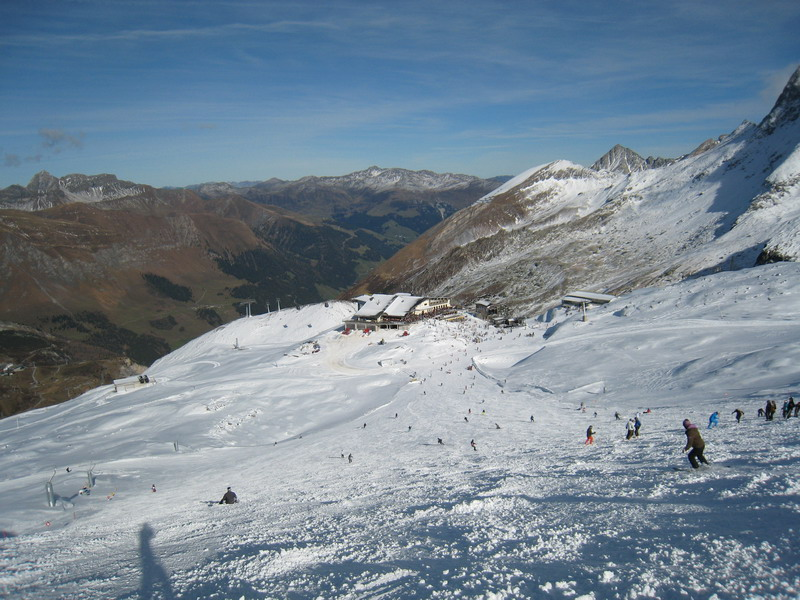
\includegraphics[width=0.31\textwidth]{./gfx/hintertux}
\caption{Tidlig sesong på Hintertux}
\end{figure}
